\begin{answer}
	\begin{figure}[H]
	\centering
	\begin{subfigure}[H]{0.45\linewidth}
		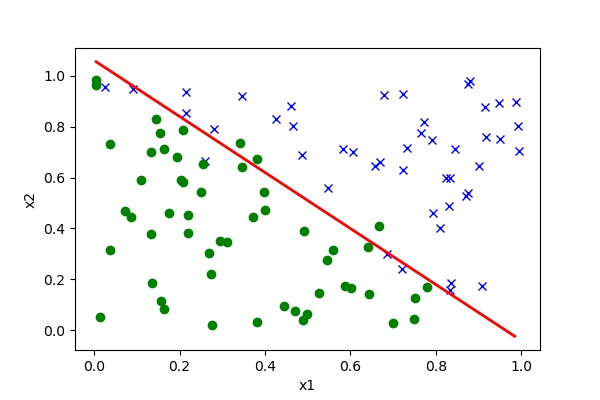
\includegraphics[width=\linewidth]{ds1_a}
		\caption{Dataset A isn't separable.}
	\end{subfigure}
	\begin{subfigure}[H]{0.45\linewidth}
		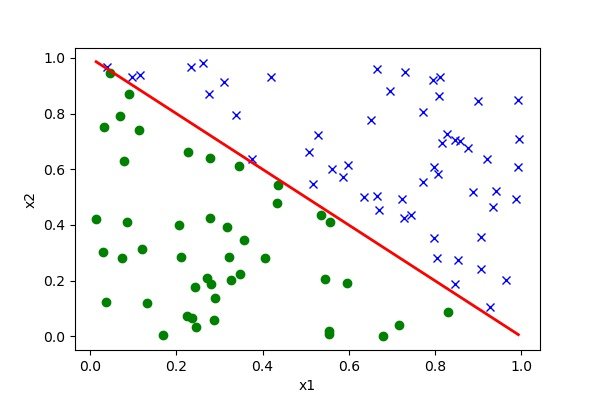
\includegraphics[width=\linewidth]{ds1_b}
		\caption{Dataset B separated by $ x_1 + x_2 = 1$.}
	\end{subfigure}
	\caption{These datasets differ in the linear separability.}
	\end{figure}
Let $\theta$ be a parameter vector such that dataset B is completely separated 
by the hyperplane $\theta^{T} x = 0$. Now, consider a parameter $\theta' = c 
\cdot \theta$. Given an example x, we observe that:
\begin{itemize}
	\item If $y=0$, then $\theta^{T} x < 0$ and its loss w.r.t. $\theta'$ is: 
	$-\log \left(\dfrac{1}{1 + \exp (-c\cdot\theta^T x)} \right)$.
	\item If $y=1$, then $\theta^T x > 0$ and its loss w.r.t. $\theta'$ is: 
	$-\log \left(1 - \dfrac{1}{1 + \exp (-c\cdot\theta^T x)} \right)$.
\end{itemize}
As $c \to \infty$, in both cases the losses are strictly decreasing without a 
bound. And so the total cost is a lower-unbounded convex function. The 
Gradient Descent will fail to converge to the global minimum since there is not 
such one. Due to inseparability, dataset A doesn't endure the above trait, our optimizer actually worked nicely. \\
\end{answer}
